\documentclass{../source/Experiment}

\major{信息工程}
\name{姚桂涛}
\title{微波传输线负载特性矢量网络分析仪测量}
\stuid{3190105597}
\college{信息与电子工程学院}
\date{\today}
\lab{东4-224}
\course{电磁场与电磁波}
\instructor{王子立}
\grades{}
\expname{微波传输线负载特性矢网测量}
\exptype{验证实验}
\partner{华天择、李宗昊}

\begin{document}
    \makecover
    \makeheader

    \section{微带传输线反射测量}
        \subsection{50$\Omega$}
            \begin{figure}[H]
                \centering
                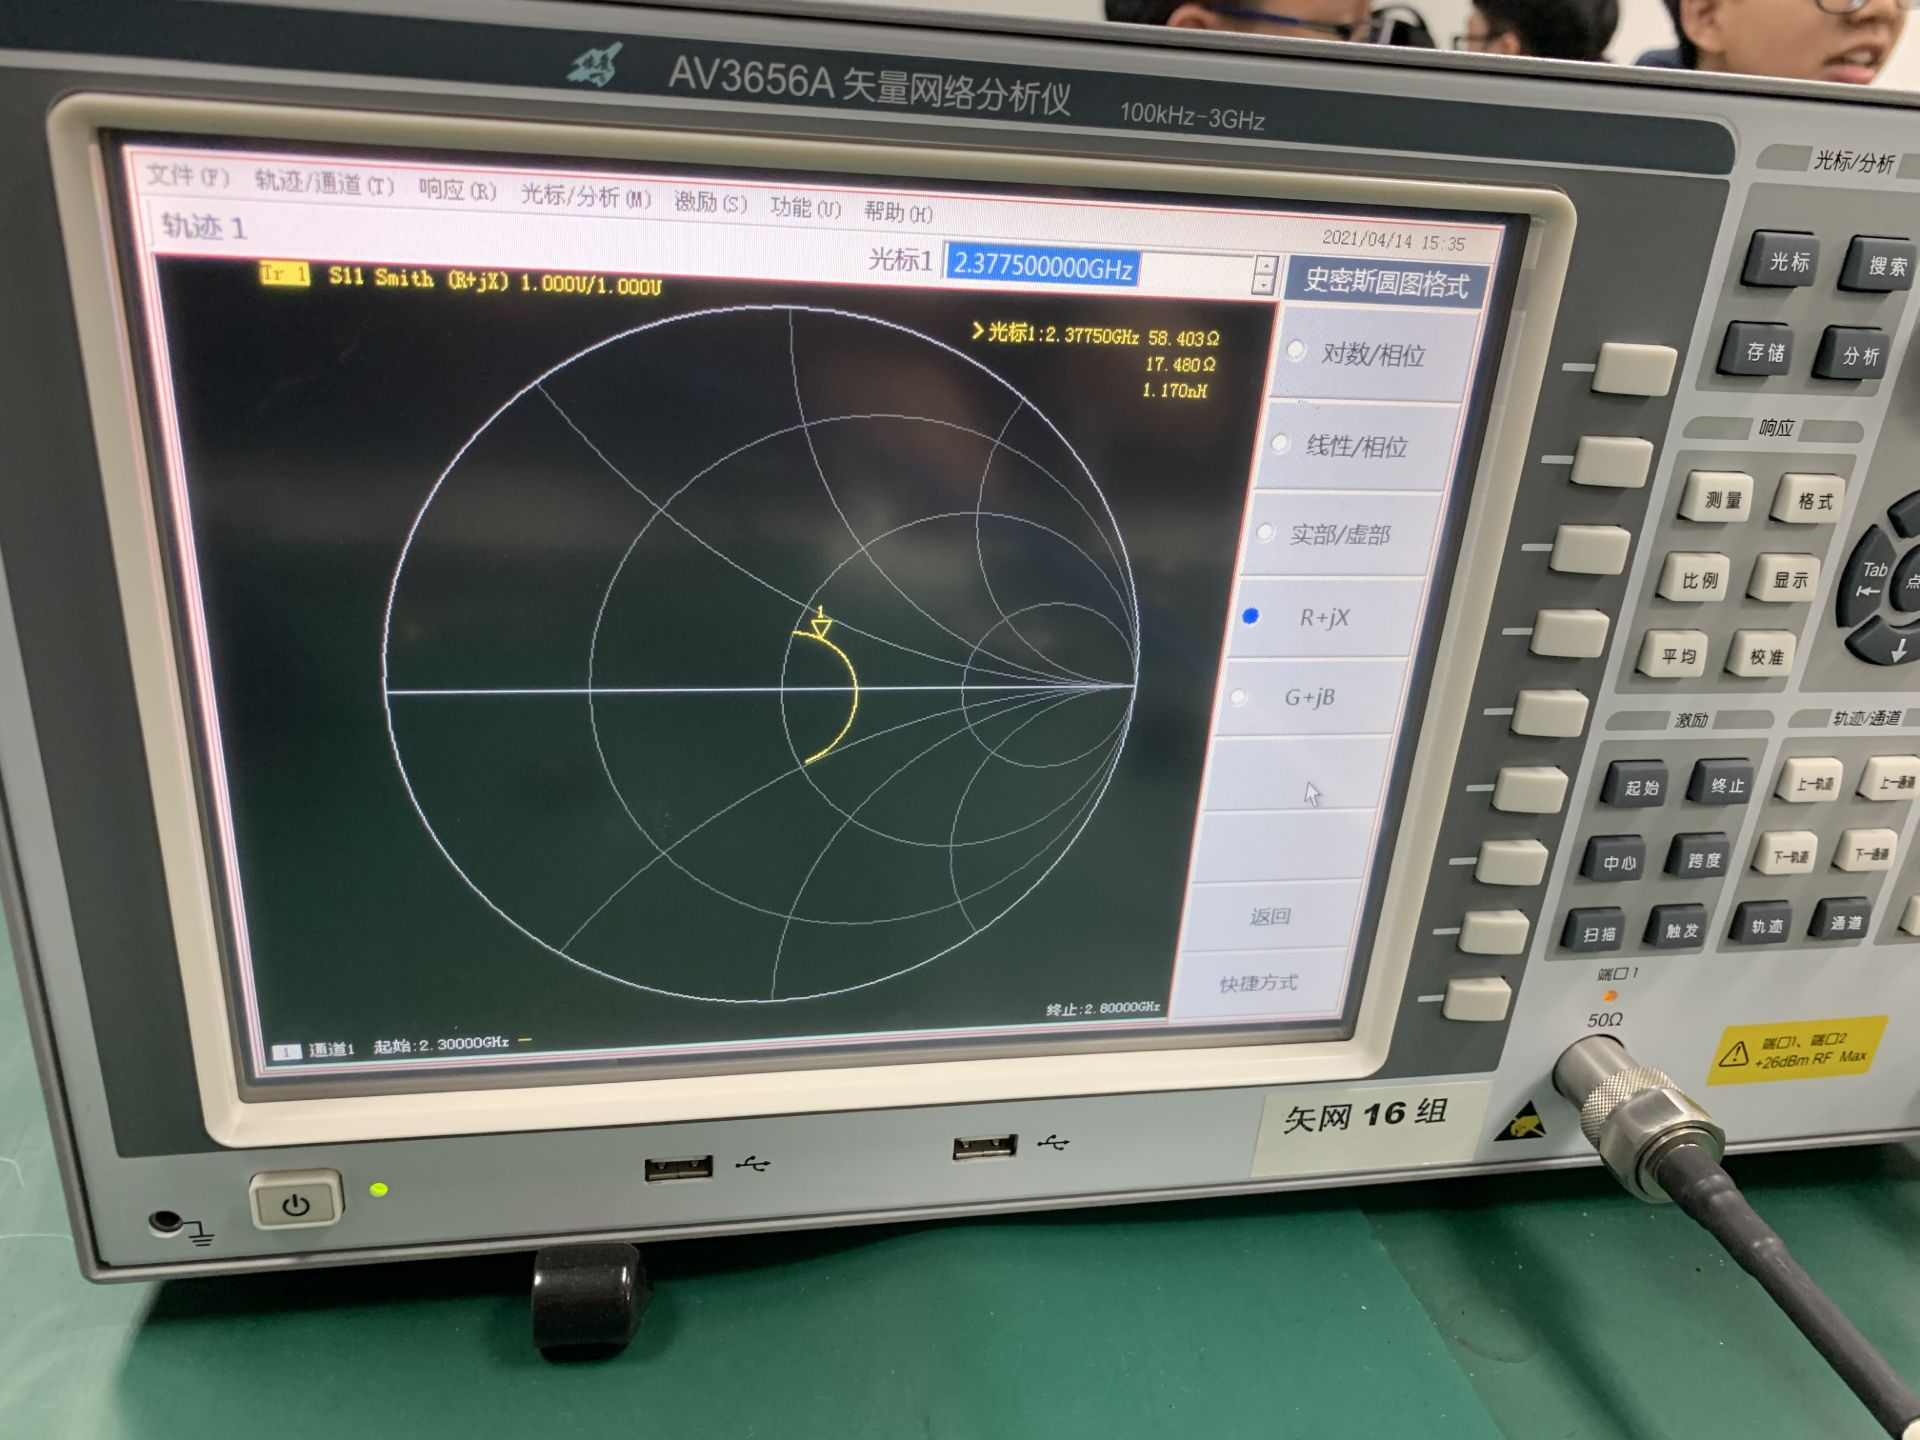
\includegraphics[width = 0.6\textwidth]{pic/49.92}
                \caption{50$\Omega$}
            \end{figure}
            $50\Omega$时,
            理论值:$$\Gamma _L = \frac{Z_{Ln}-1}{Z_{Ln}+1} = \frac{Z_L - Z_0}{Z_L - Z_0} = 0$$
            
            测量值:
            \begin{table}[H]
                \centering
                \begin{tabular}{|c|c|c|c|c|c|}
                \hline
                频率GHz  & $Re(Z_{in})$ & $Im(Z_{in})$ & $\Gamma _R$ & $\Gamma _I$ & $\Gamma _理论$ \\ \hline
                2.5000 & 60.667     & 17.453     & 0.118       & 0.169       & 0            \\ \hline
                2.3775 & 58.403     & 17.480     & 0.101       & 0.169       & 0            \\ \hline
                \end{tabular}
            \end{table}
        比较测量值和理论值可以发现,测量值和理论值之间有一定的误差,并且发现当频率减小时,更加接近理论值。分析可能是因为电缆的$L$比理论的$\lambda /2$大导致


        \subsection{0$\Omega$}
            \begin{figure}[H]
                \centering
                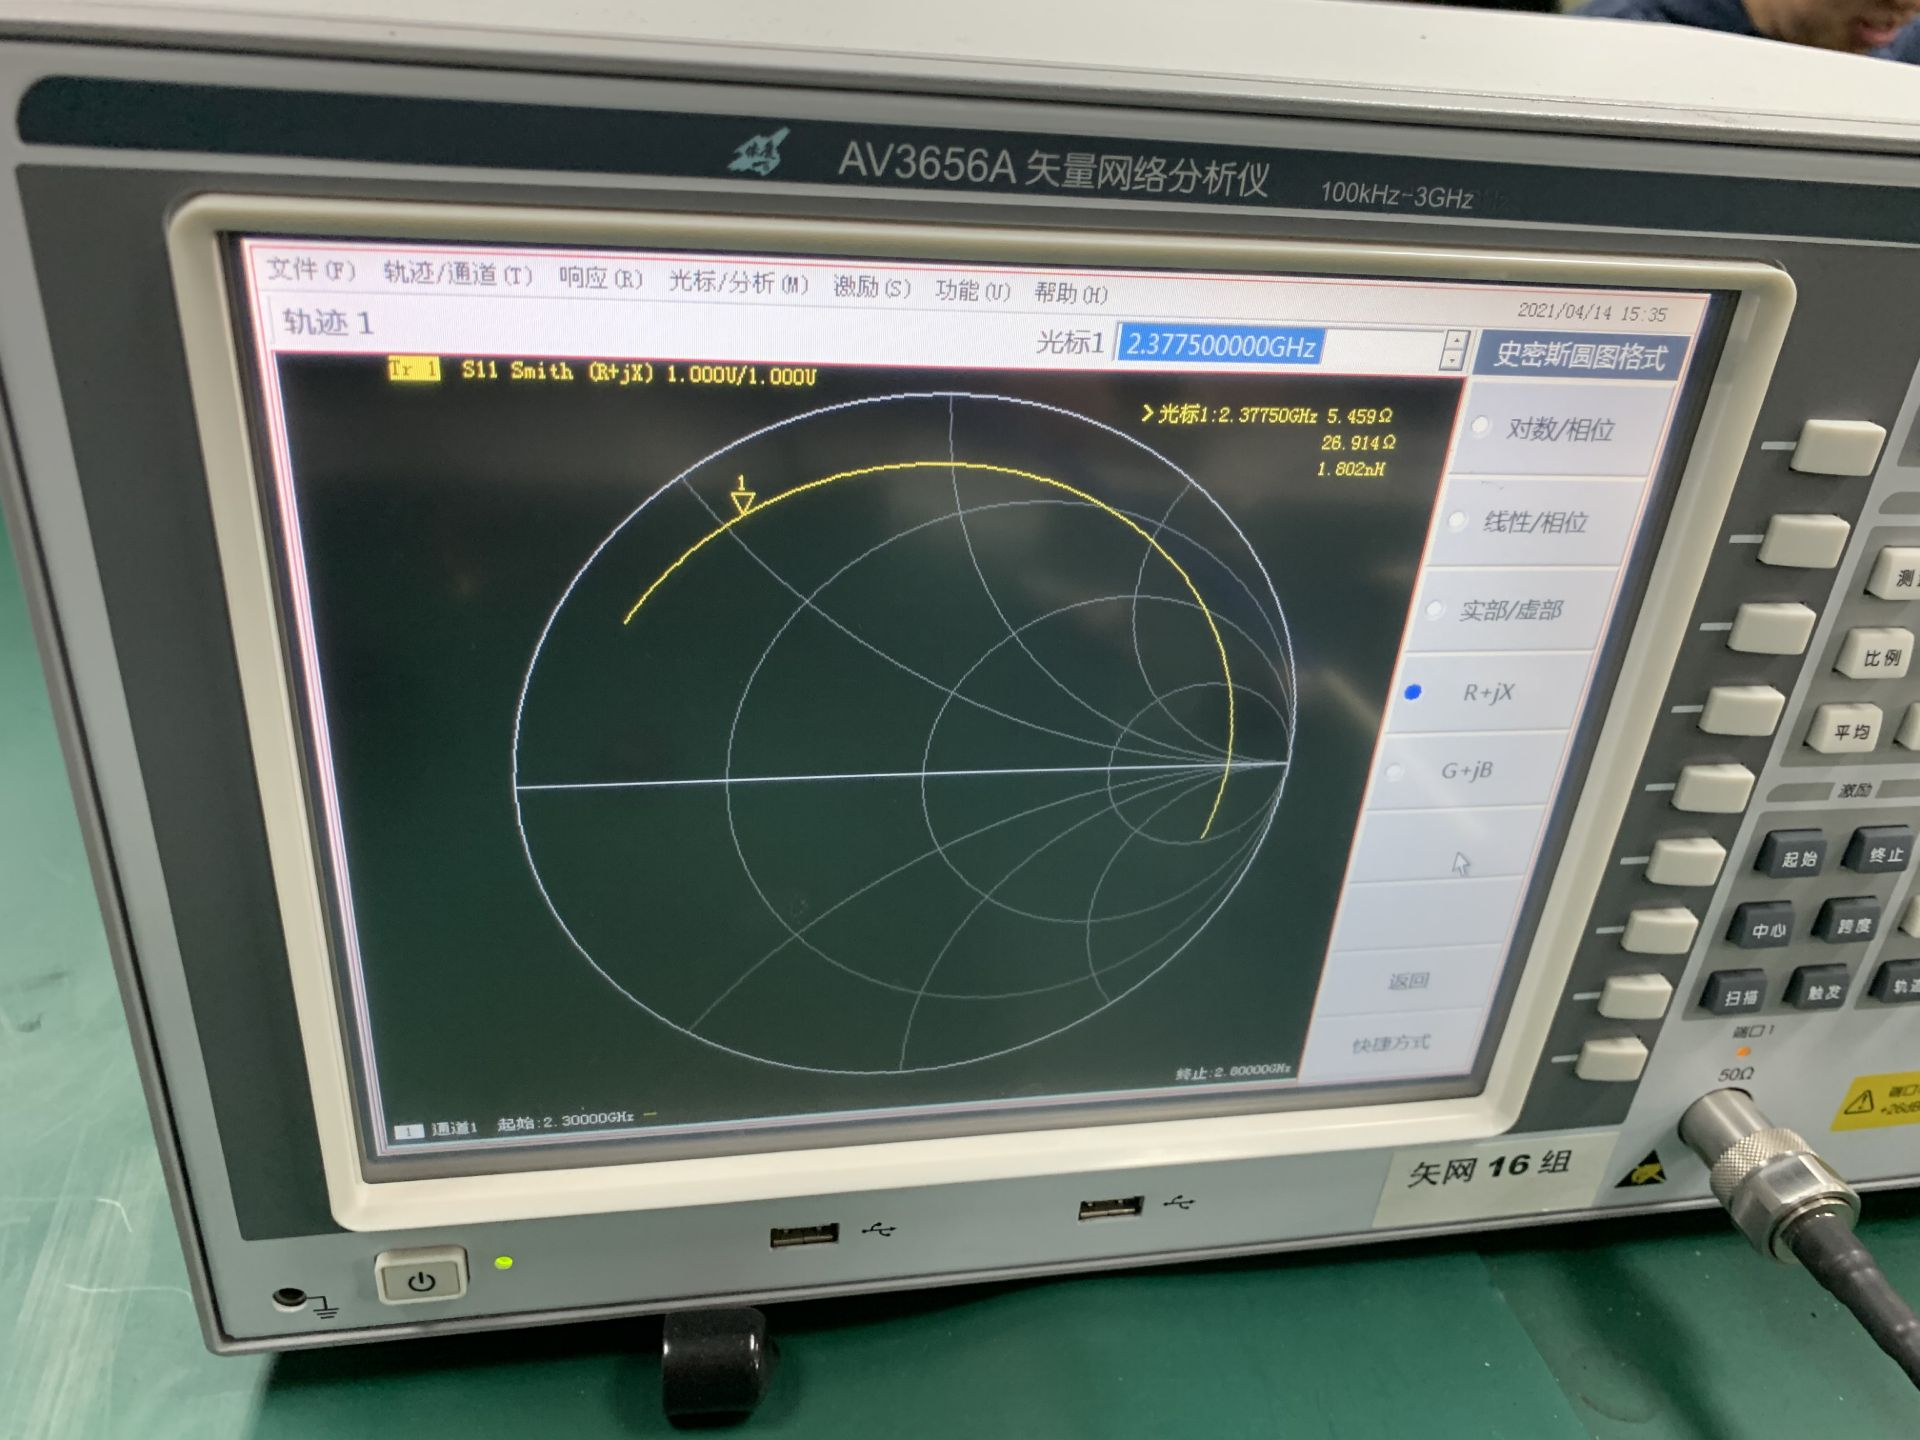
\includegraphics[width = 0.6\textwidth]{pic/02}
                \caption{0$\Omega$}
            \end{figure}
        理论值:$$\Gamma _L = \frac{Z_{Ln}-1}{Z_{Ln}+1} = \frac{Z_L - Z_0}{Z_L - Z_0} = -1$$
        
        测量值:
        \begin{table}[H]
            \centering
            \begin{tabular}{|c|c|c|c|c|c|}
            \hline
            频率GHz  & $Re(Z_{in})$ & $Im(Z_{in})$ & $\Gamma _R$ & $\Gamma _I$ & $\Gamma _理论$ \\ \hline
            2.5000 & 5.970      & 28.442     & -0.420      & 0.086       & -1           \\ \hline
            2.3775 & 5.459      & 26.914     & -0.459      & 0.077       & 0            \\ \hline
            \end{tabular}
        \end{table}
            
        比较测量值和理论值可以发现,测量值和理论值之间有一定的误差,并且发现当频率减小时,更加接近理论值。分析可能是因为电缆的$L$比理论的$\lambda /2$大导致

        \subsection{电容}
            \begin{figure}[H]
                \centering
                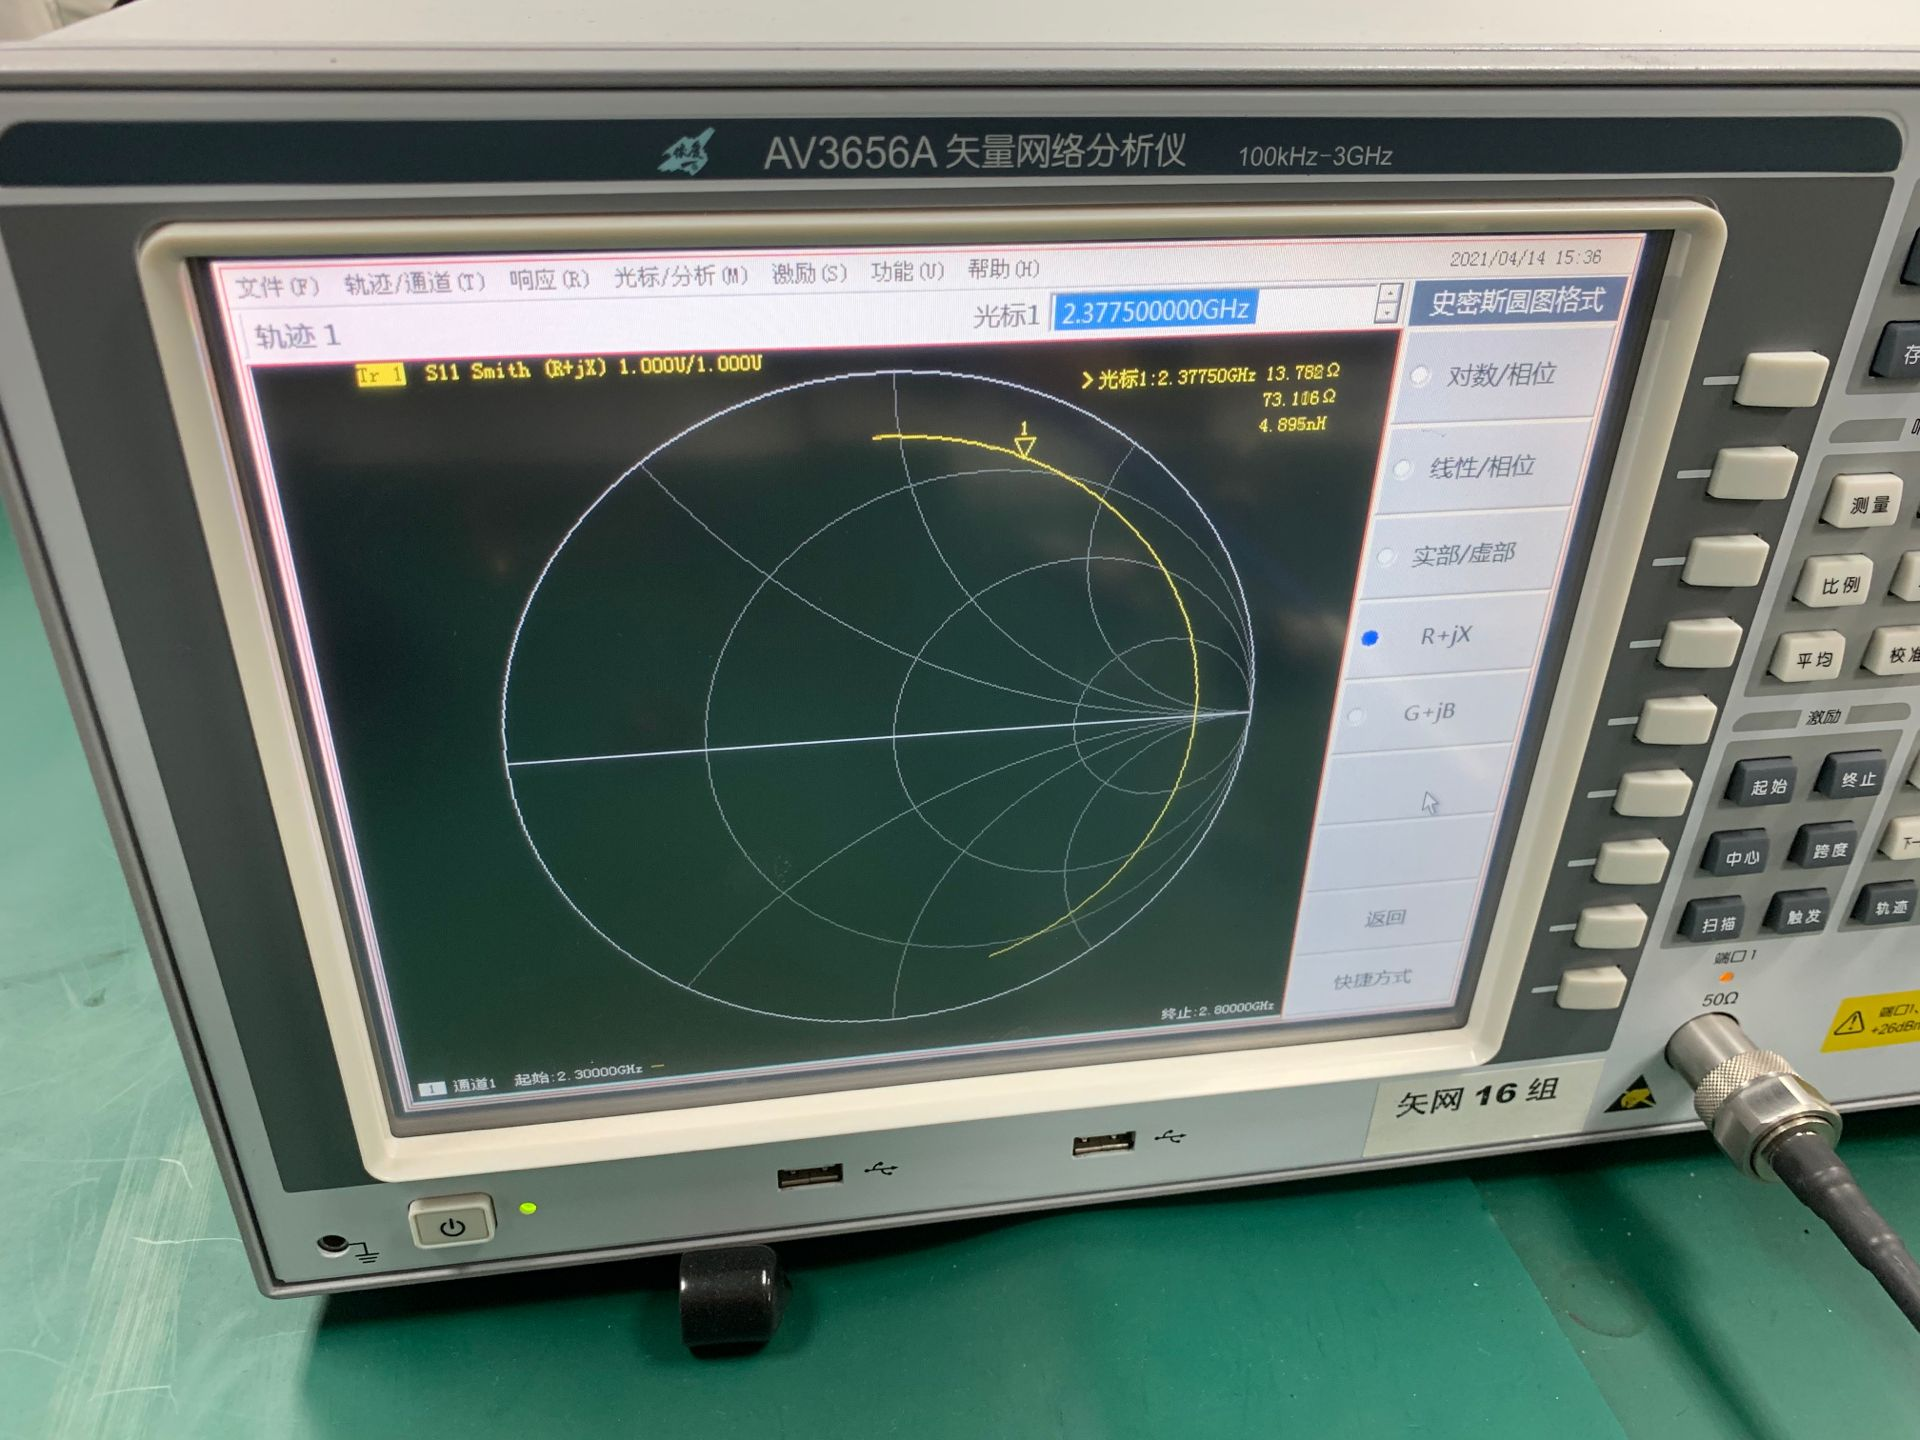
\includegraphics[width = 0.6\textwidth]{pic/L2}
                \caption{电容}
            \end{figure}
            理论值:$$\Gamma _L = \frac{Z_{Ln}-1}{Z_{Ln}+1} = \frac{Z_L - Z_0}{Z_L - Z_0} = 0.2369 −
            0.9715i$$
            
            测量值:
            \begin{table}[H]
                \centering
                \begin{tabular}{|c|c|c|c|c|c|}
                \hline
                频率GHz  & $Re(Z_{in})$ & $Im(Z_{in})$ & $\Gamma _R$ & $\Gamma _I$ & $\Gamma _理论$ \\ \hline
                2.5000 & 17.887     & 89.632     & 0.463       & 0.254       & 0.036        \\ \hline
                2.3775 & 13.782     & 73.116     & 0.322       & 0.214       & 0.999        \\ \hline
                \end{tabular}
            \end{table}
            比较测量值和理论值可以发现,测量值和理论值之间有一定的误差,并且发现实部的误差更小。

        \subsection{电感}
            \begin{figure}[H]
                \centering
                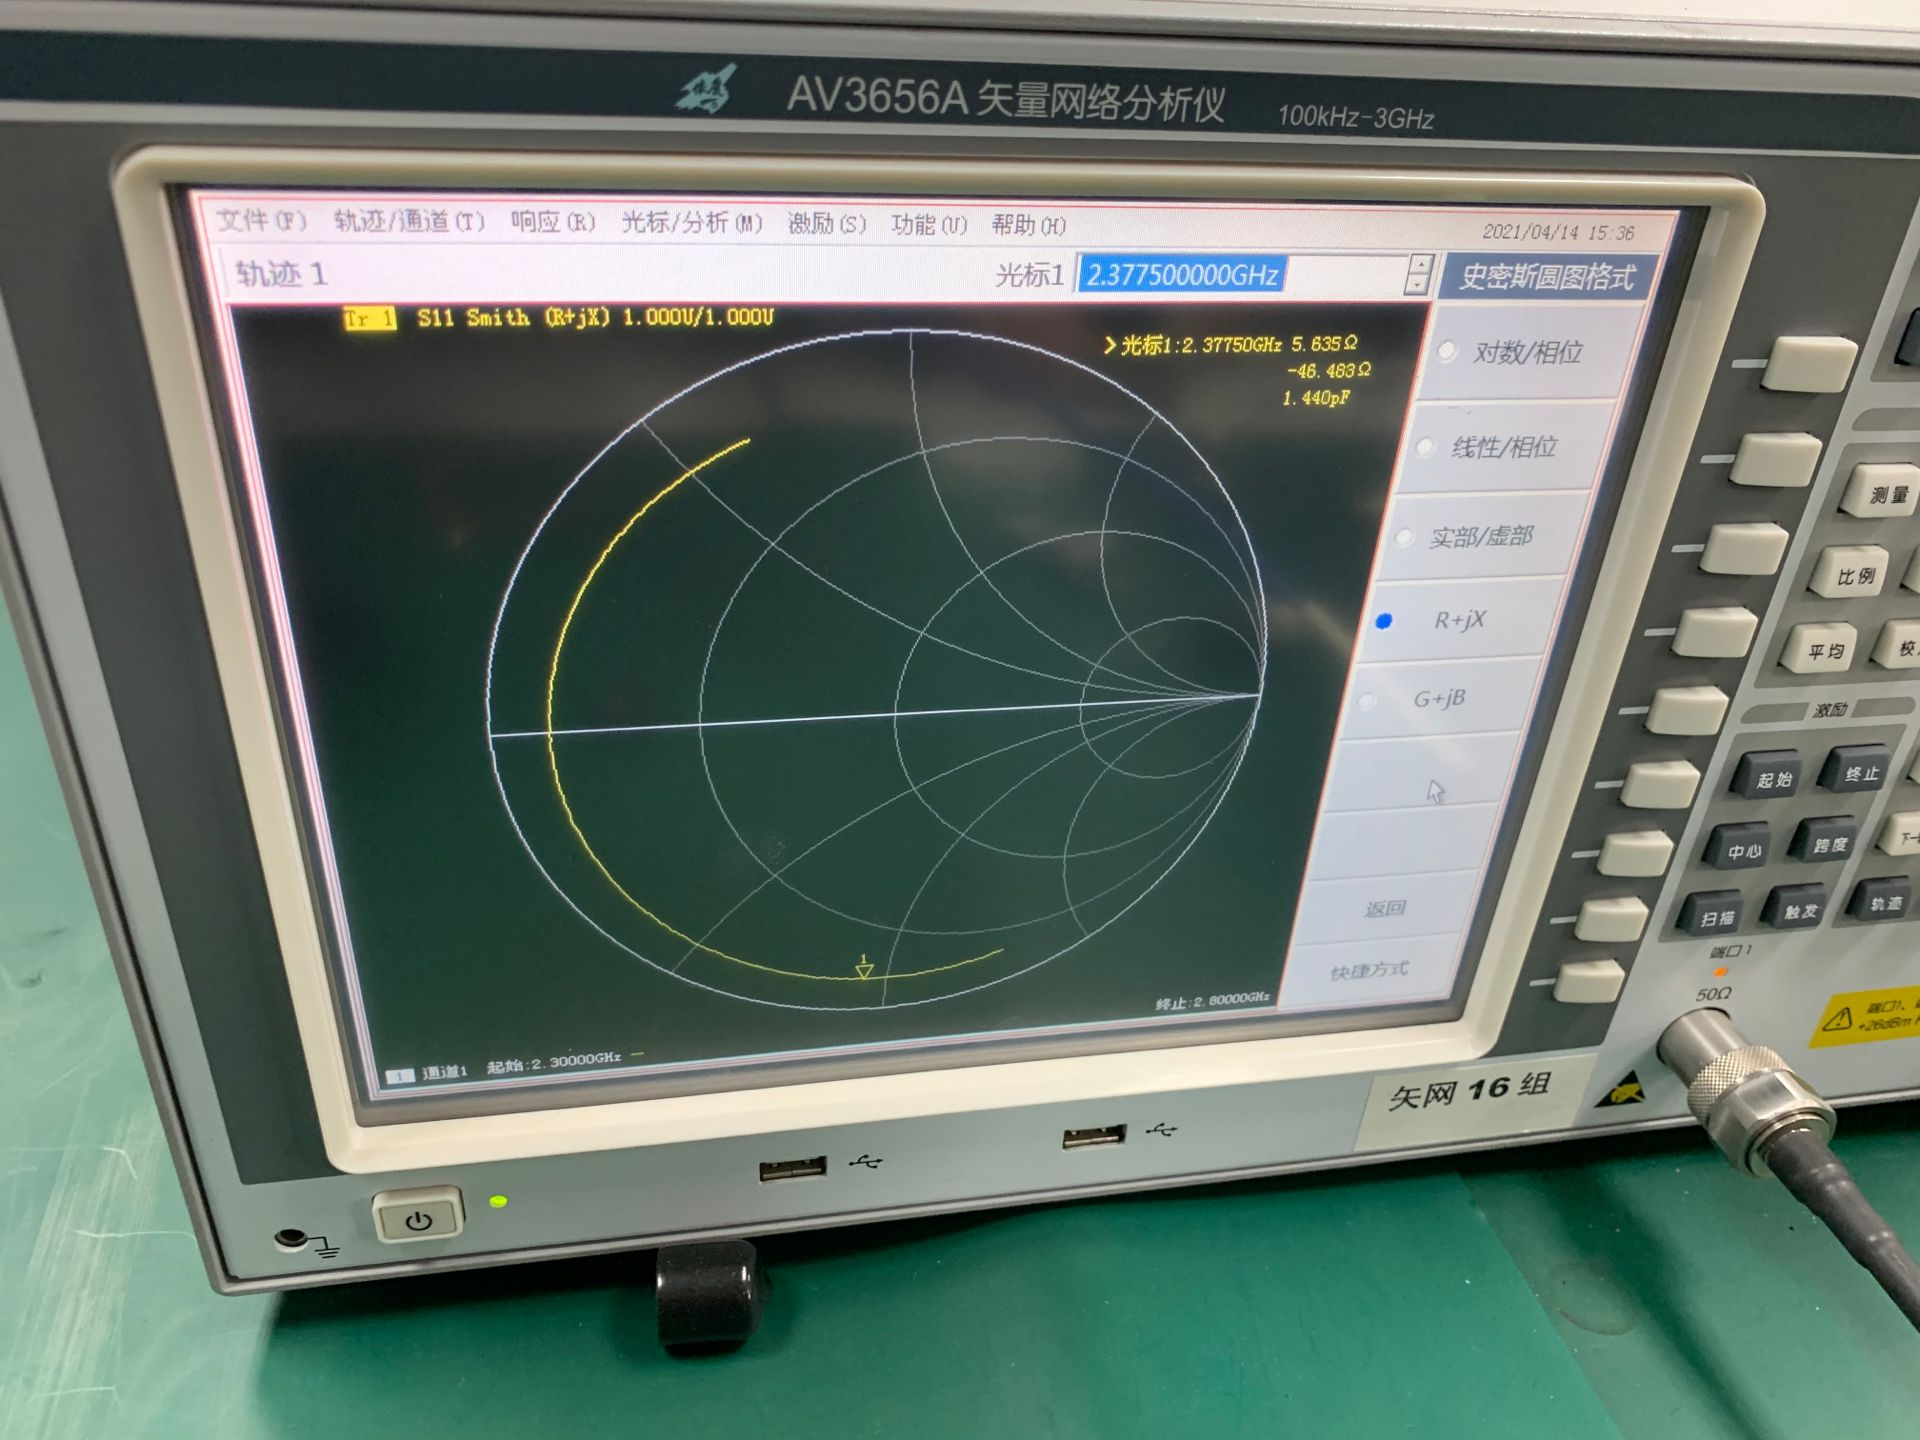
\includegraphics[width = 0.6\textwidth]{pic/C2}
                \caption{电感}
            \end{figure}
            理论值:$$\Gamma _L = \frac{Z_{Ln}-1}{Z_{Ln}+1} = \frac{Z_L - Z_0}{Z_L - Z_0} = 0.036 +
            0.999i$$
            
            测量值:
            \begin{table}[H]
                \centering
                \begin{tabular}{|c|c|c|c|c|c|}
                \hline
                频率GHz  & $Re(Z_{in})$ & $Im(Z_{in})$ & $\Gamma _R$ & $\Gamma _I$ & $\Gamma _理论$ \\ \hline
                2.5000 & 5.997      & -43.478    & -0.114      & -0.104      & 0.237        \\ \hline
                2.3775 & 5.635      & -46.488    & -0.058      & -0.100      & 0.972        \\ \hline
                \end{tabular}
            \end{table}

            比较测量值和理论值可以发现,相较于其他组的结果,电感的误差比较大。分析可能是操作原因导致的误差。
    \section{天线测量}
        \begin{figure}[H]
            \centering
            \begin{minipage}[t]{0.3\textwidth}
                \centering
                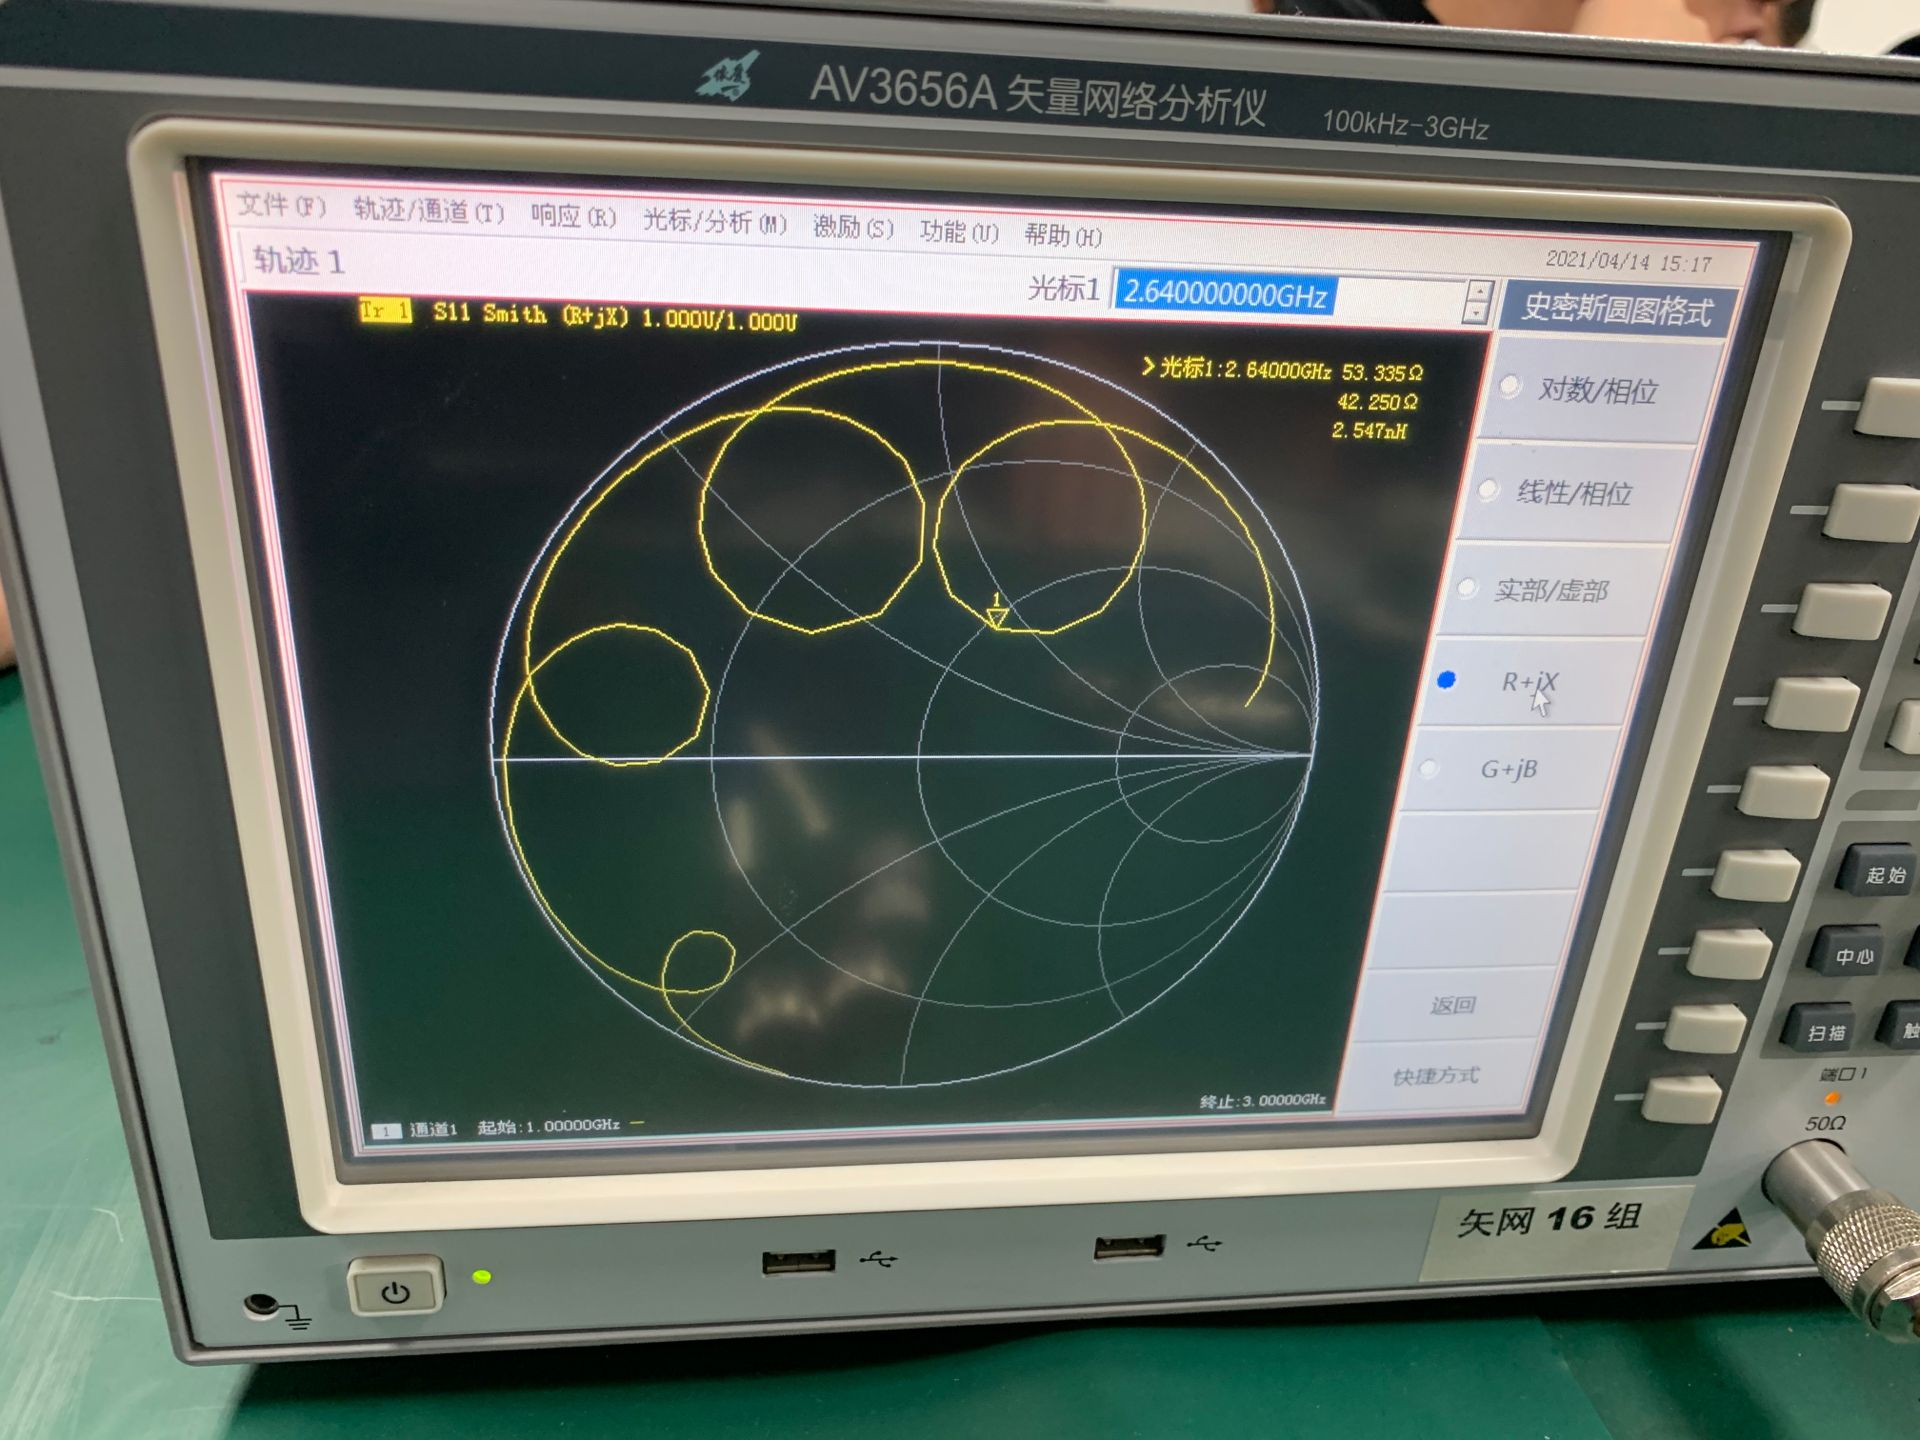
\includegraphics[width=1\textwidth]{pic/天线}
                \caption{天线}
            \end{minipage}
            \begin{minipage}[t]{0.3\textwidth}
                \centering
                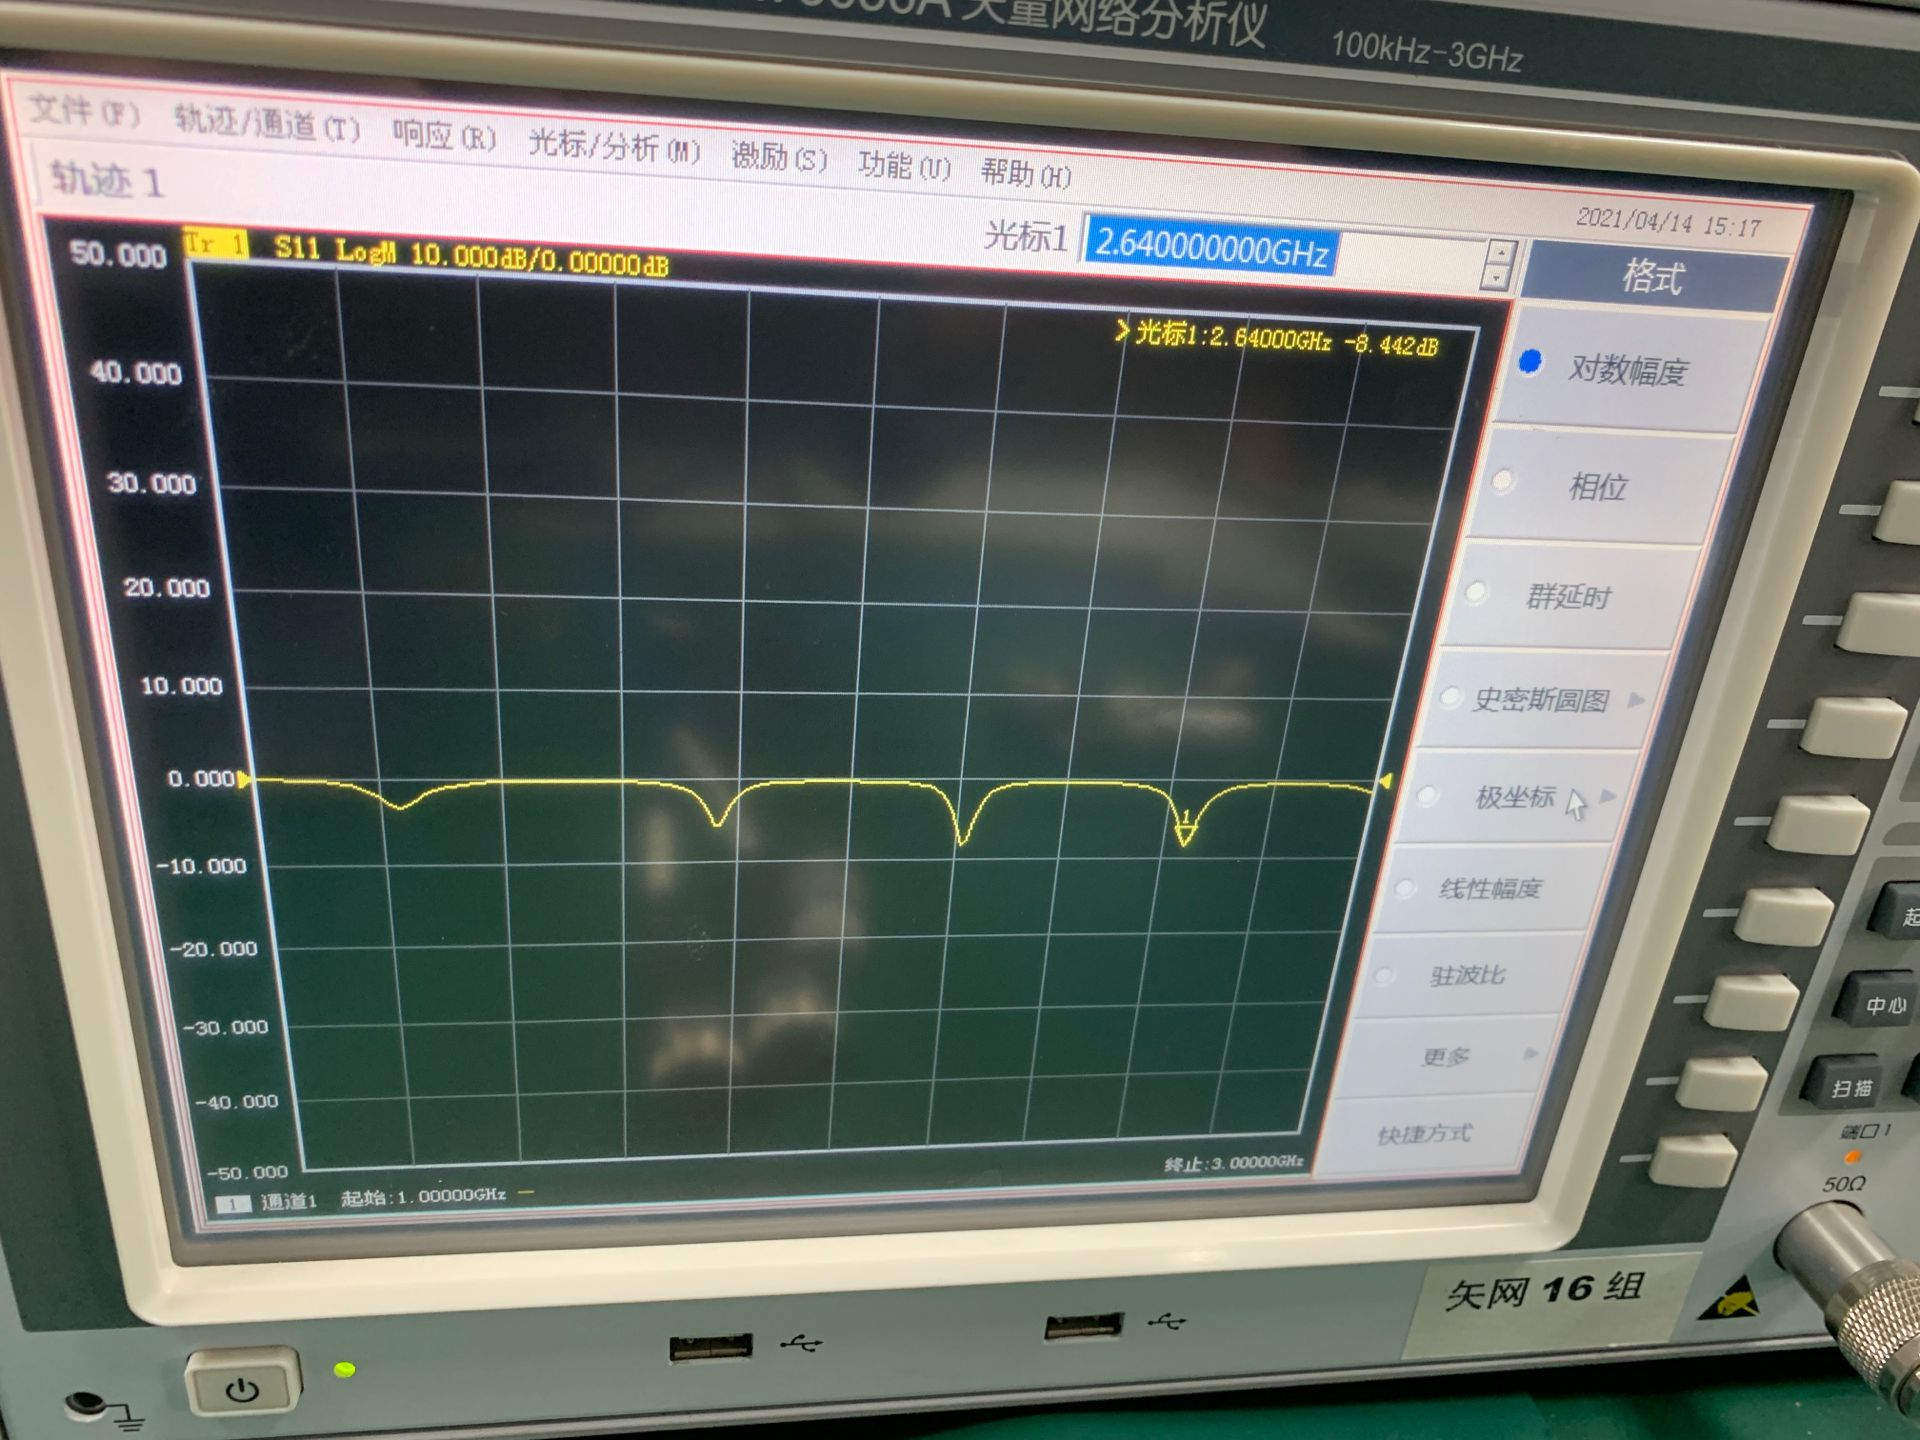
\includegraphics[width=1\textwidth]{pic/吸收峰}
                \caption{吸收峰}
            \end{minipage}
            \begin{minipage}[t]{0.3\textwidth}
                \centering
                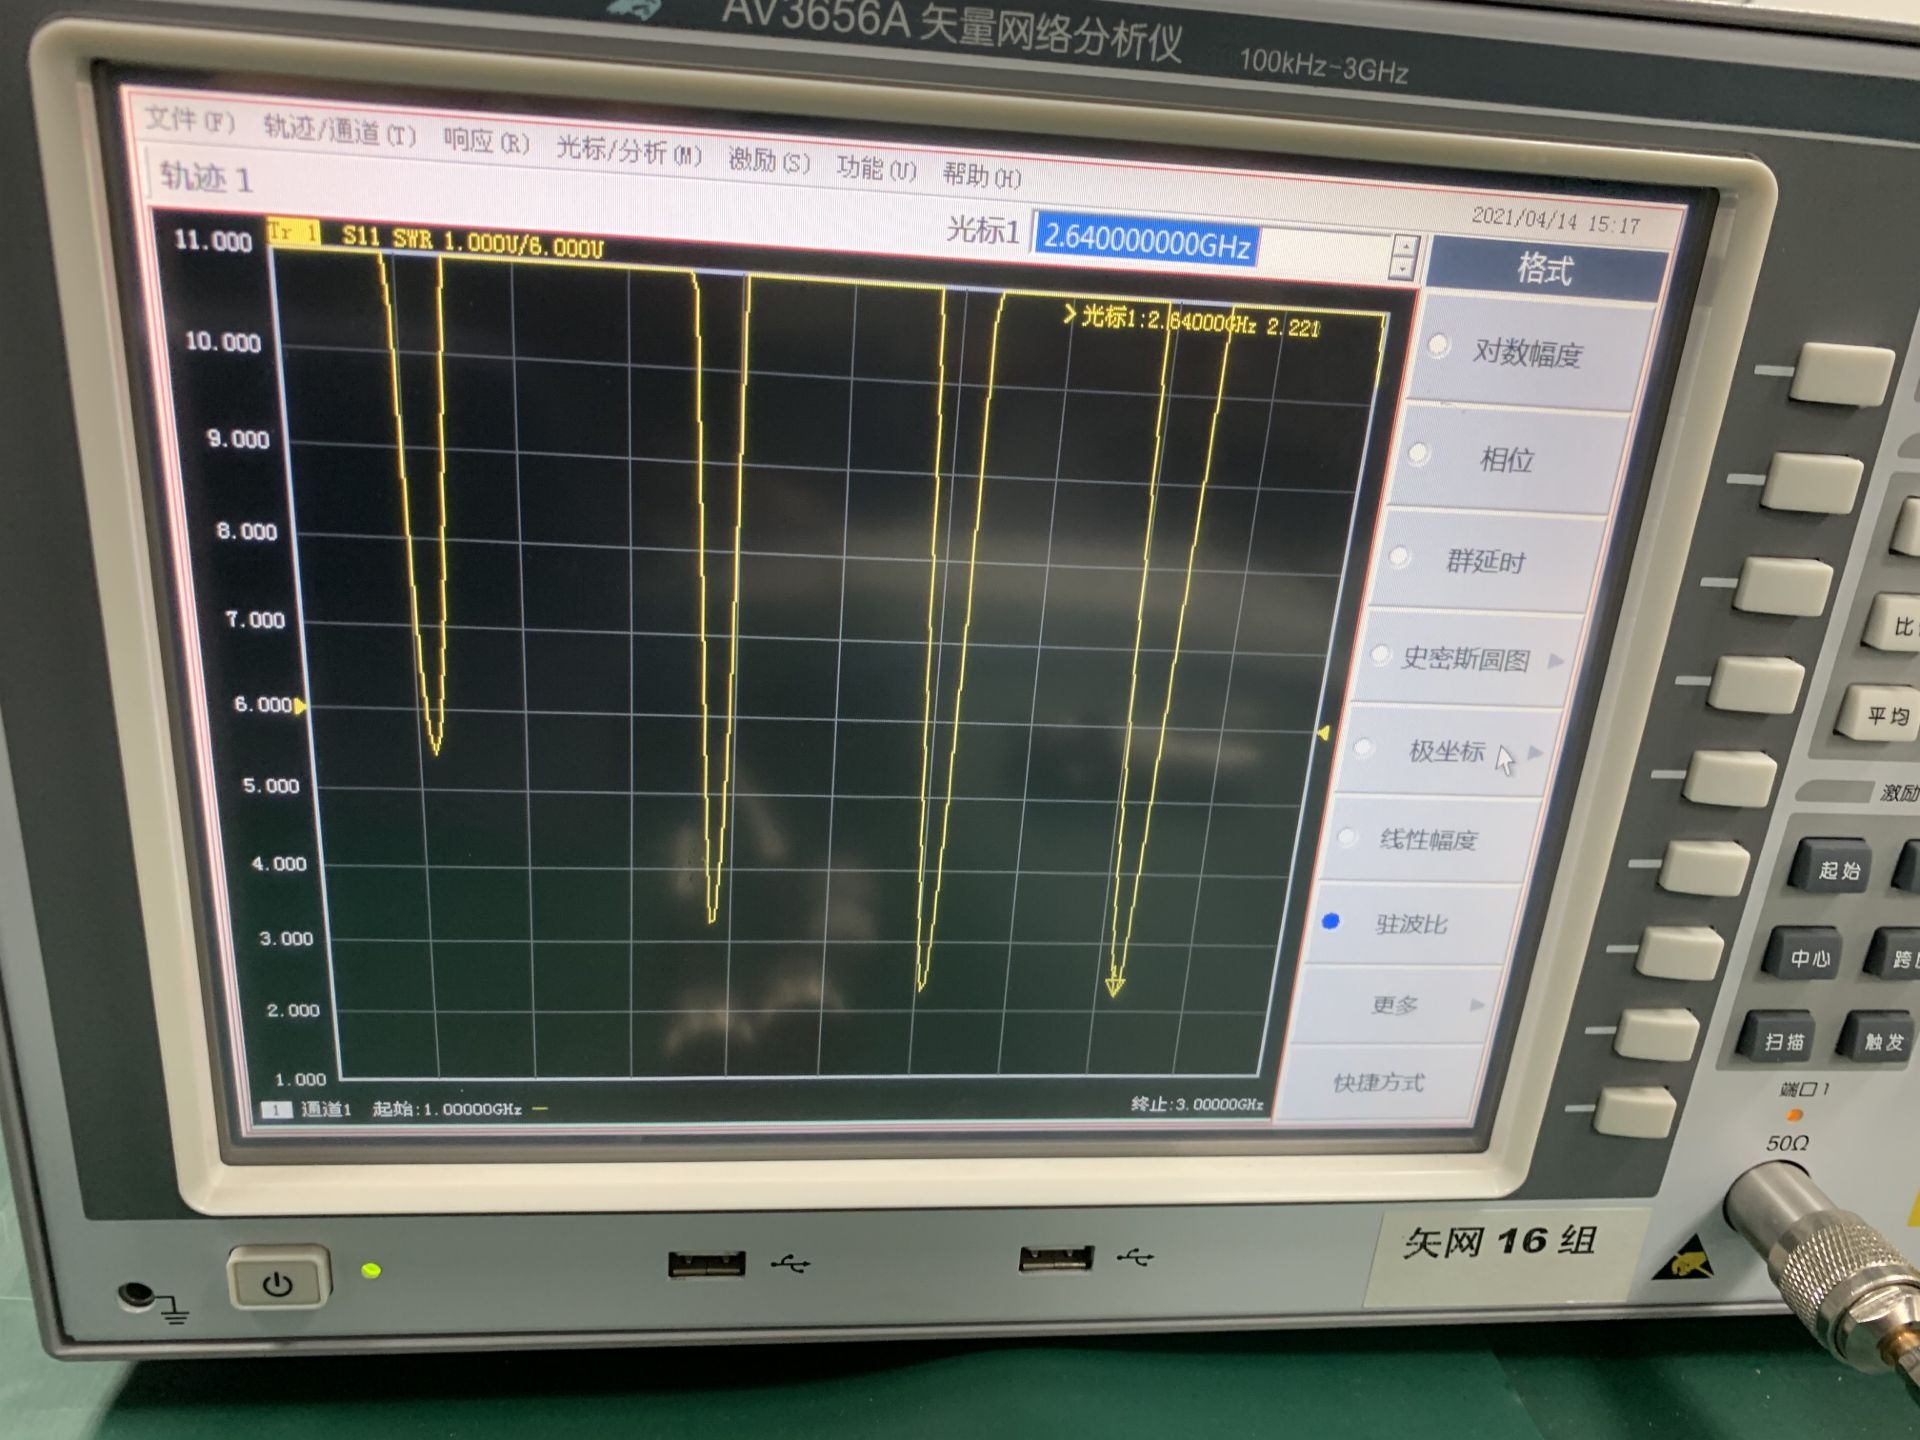
\includegraphics[width=1\textwidth]{pic/驻波系数}
                \caption{驻波系数}
            \end{minipage}
        \end{figure}

        从驻波系数来看,驻波系数几乎没有在1.5以下,说明这个天线反射特性并不是很好,可能是因为设置的工作频率为合理设置。

    \section{微带滤波器测量}

        \begin{figure}[H]
            \centering
            \begin{minipage}[t]{0.48\textwidth}
                \centering
                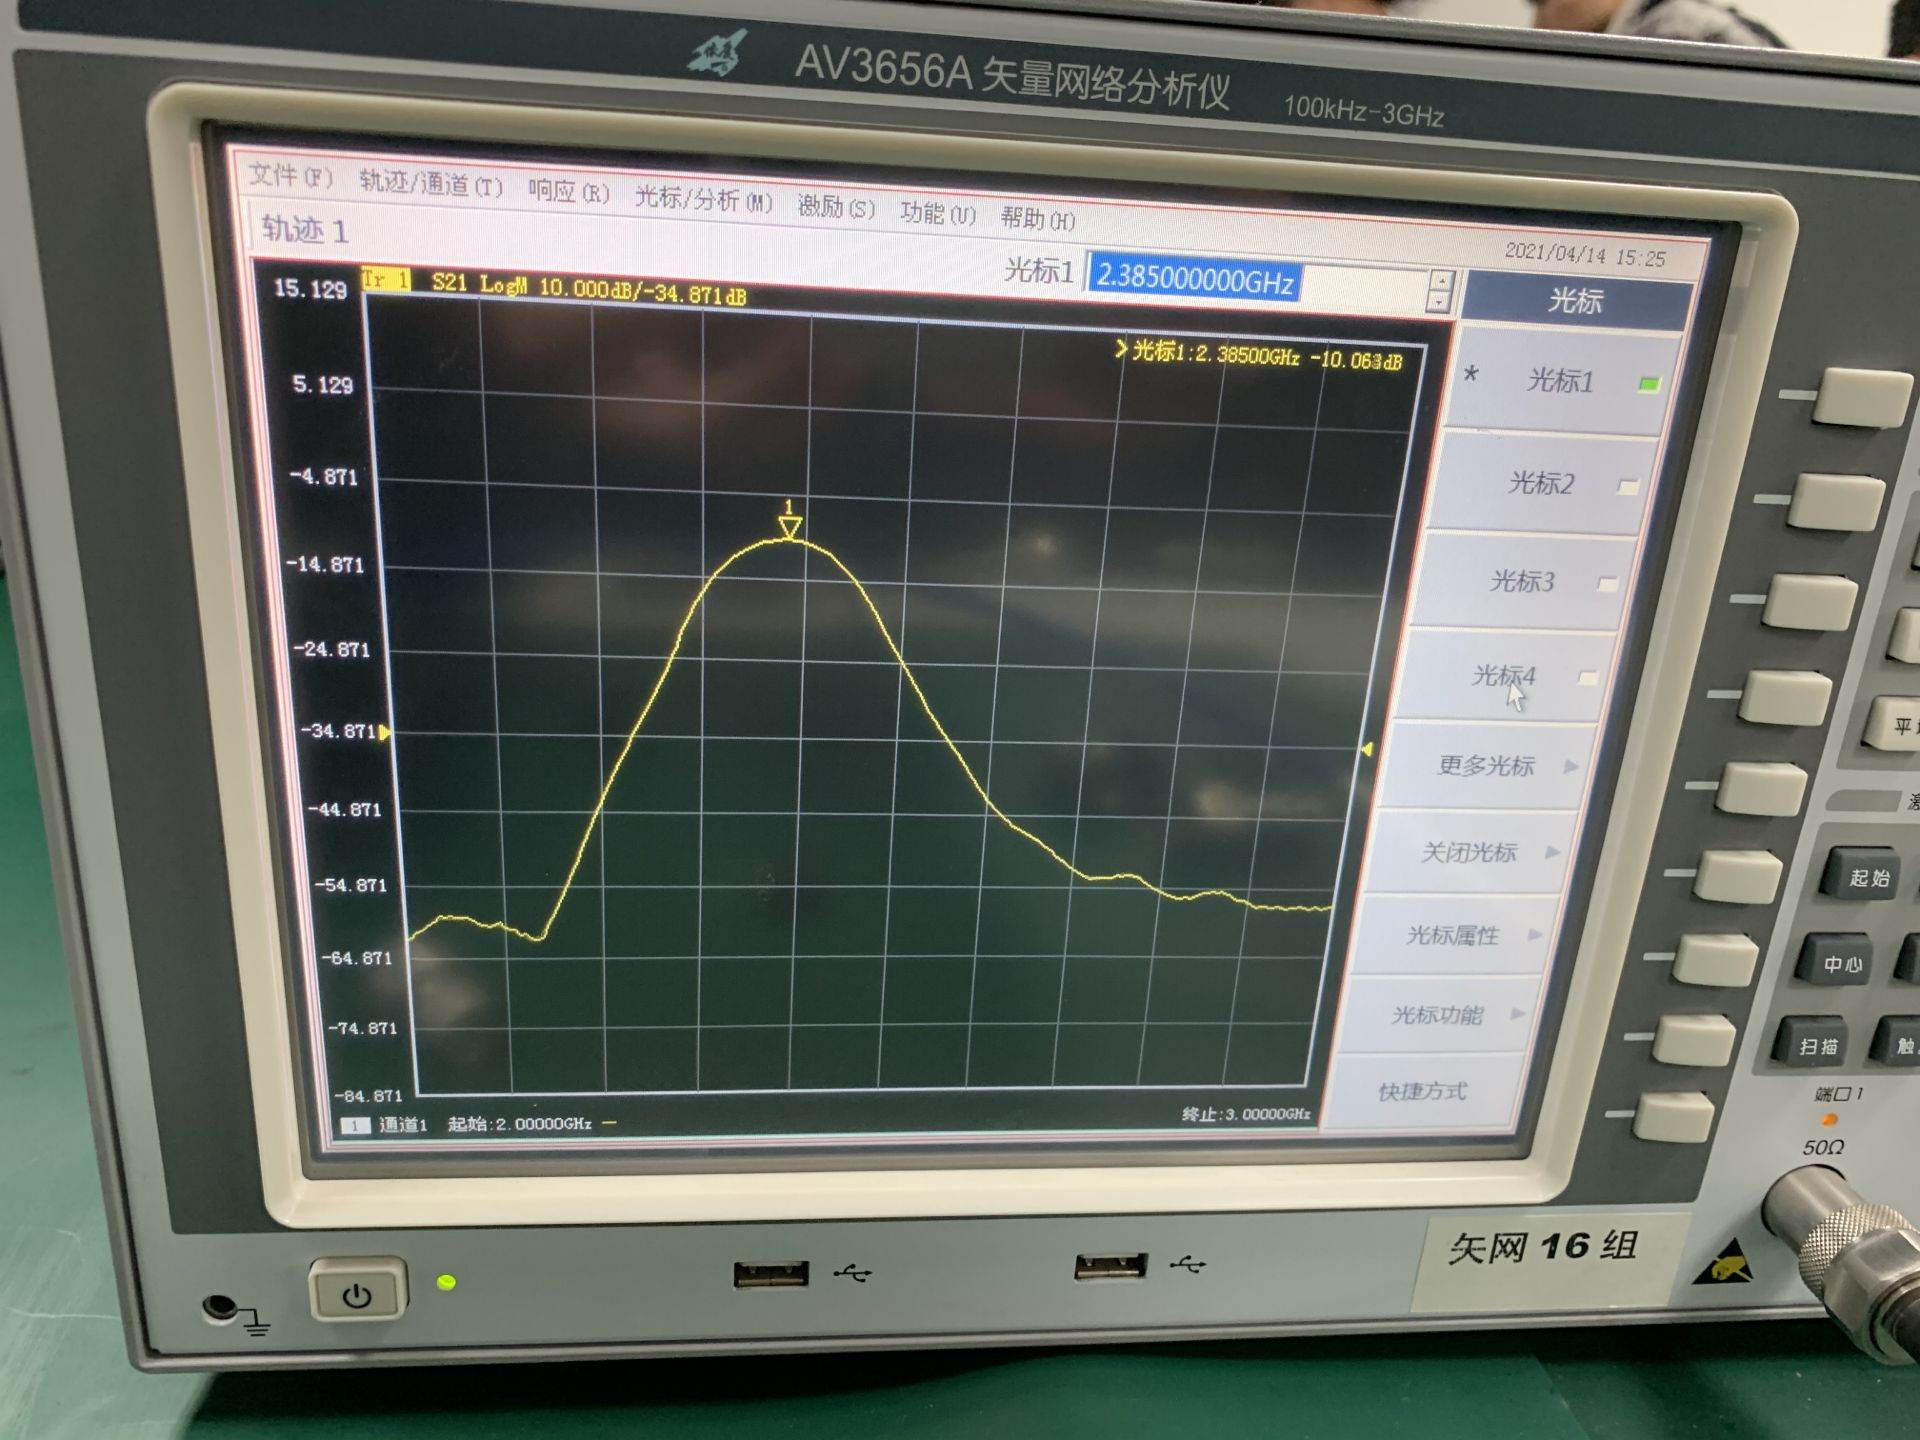
\includegraphics[width=1\textwidth]{pic/滤波特性}
                \caption{滤波特性}
            \end{minipage}
            \begin{minipage}[t]{0.48\textwidth}
                \centering
                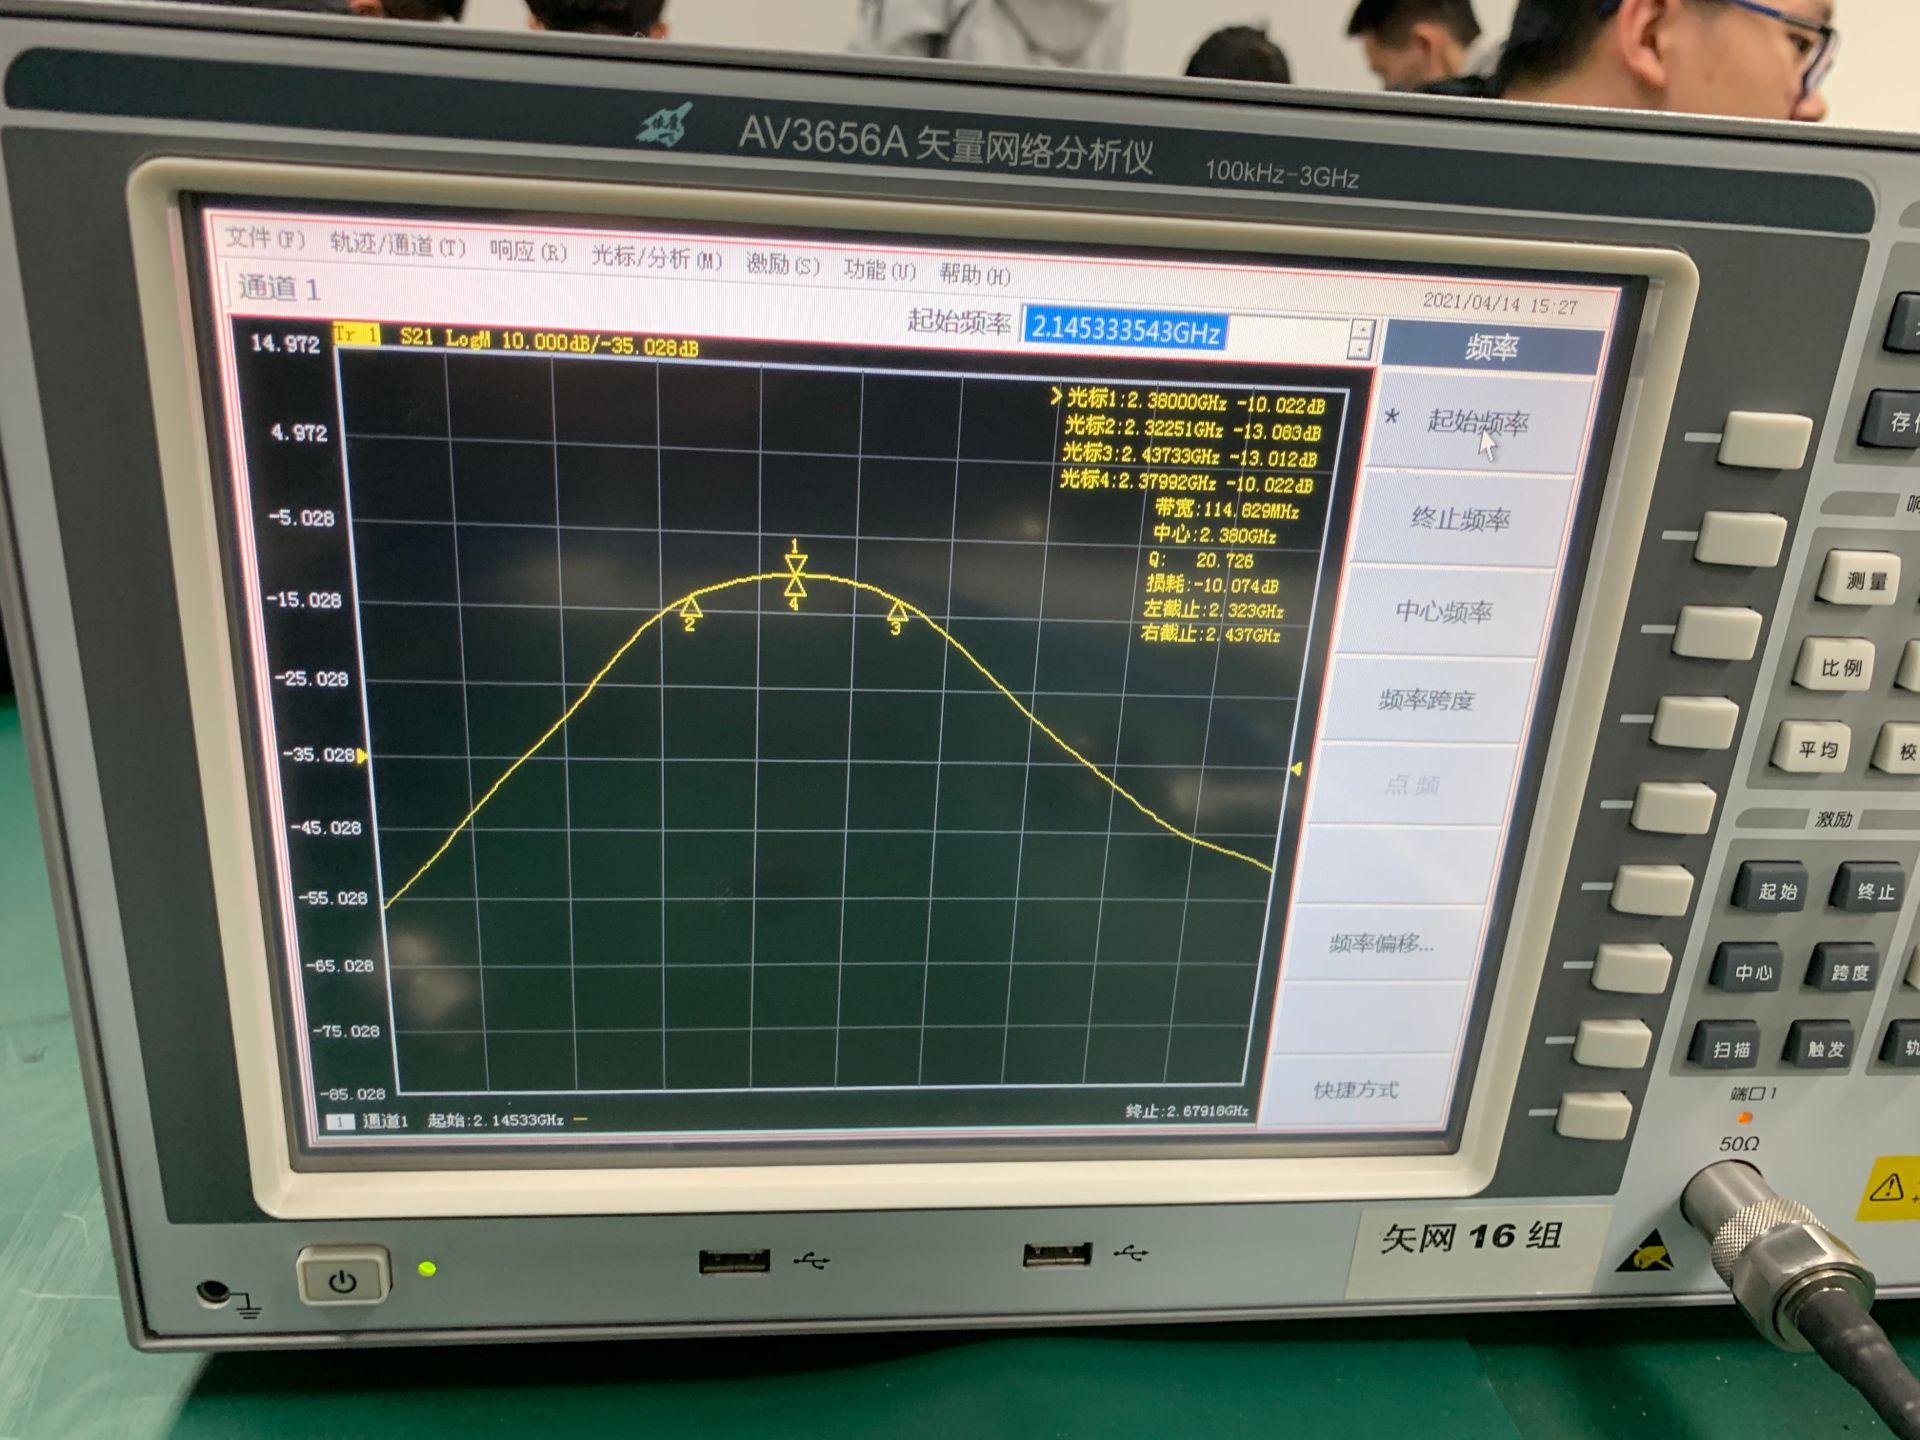
\includegraphics[width=1\textwidth]{pic/带宽}
                \caption{带宽}
            \end{minipage}
        \end{figure}

        \begin{figure}[H]
            \centering
            \begin{minipage}[t]{0.48\textwidth}
                \centering
                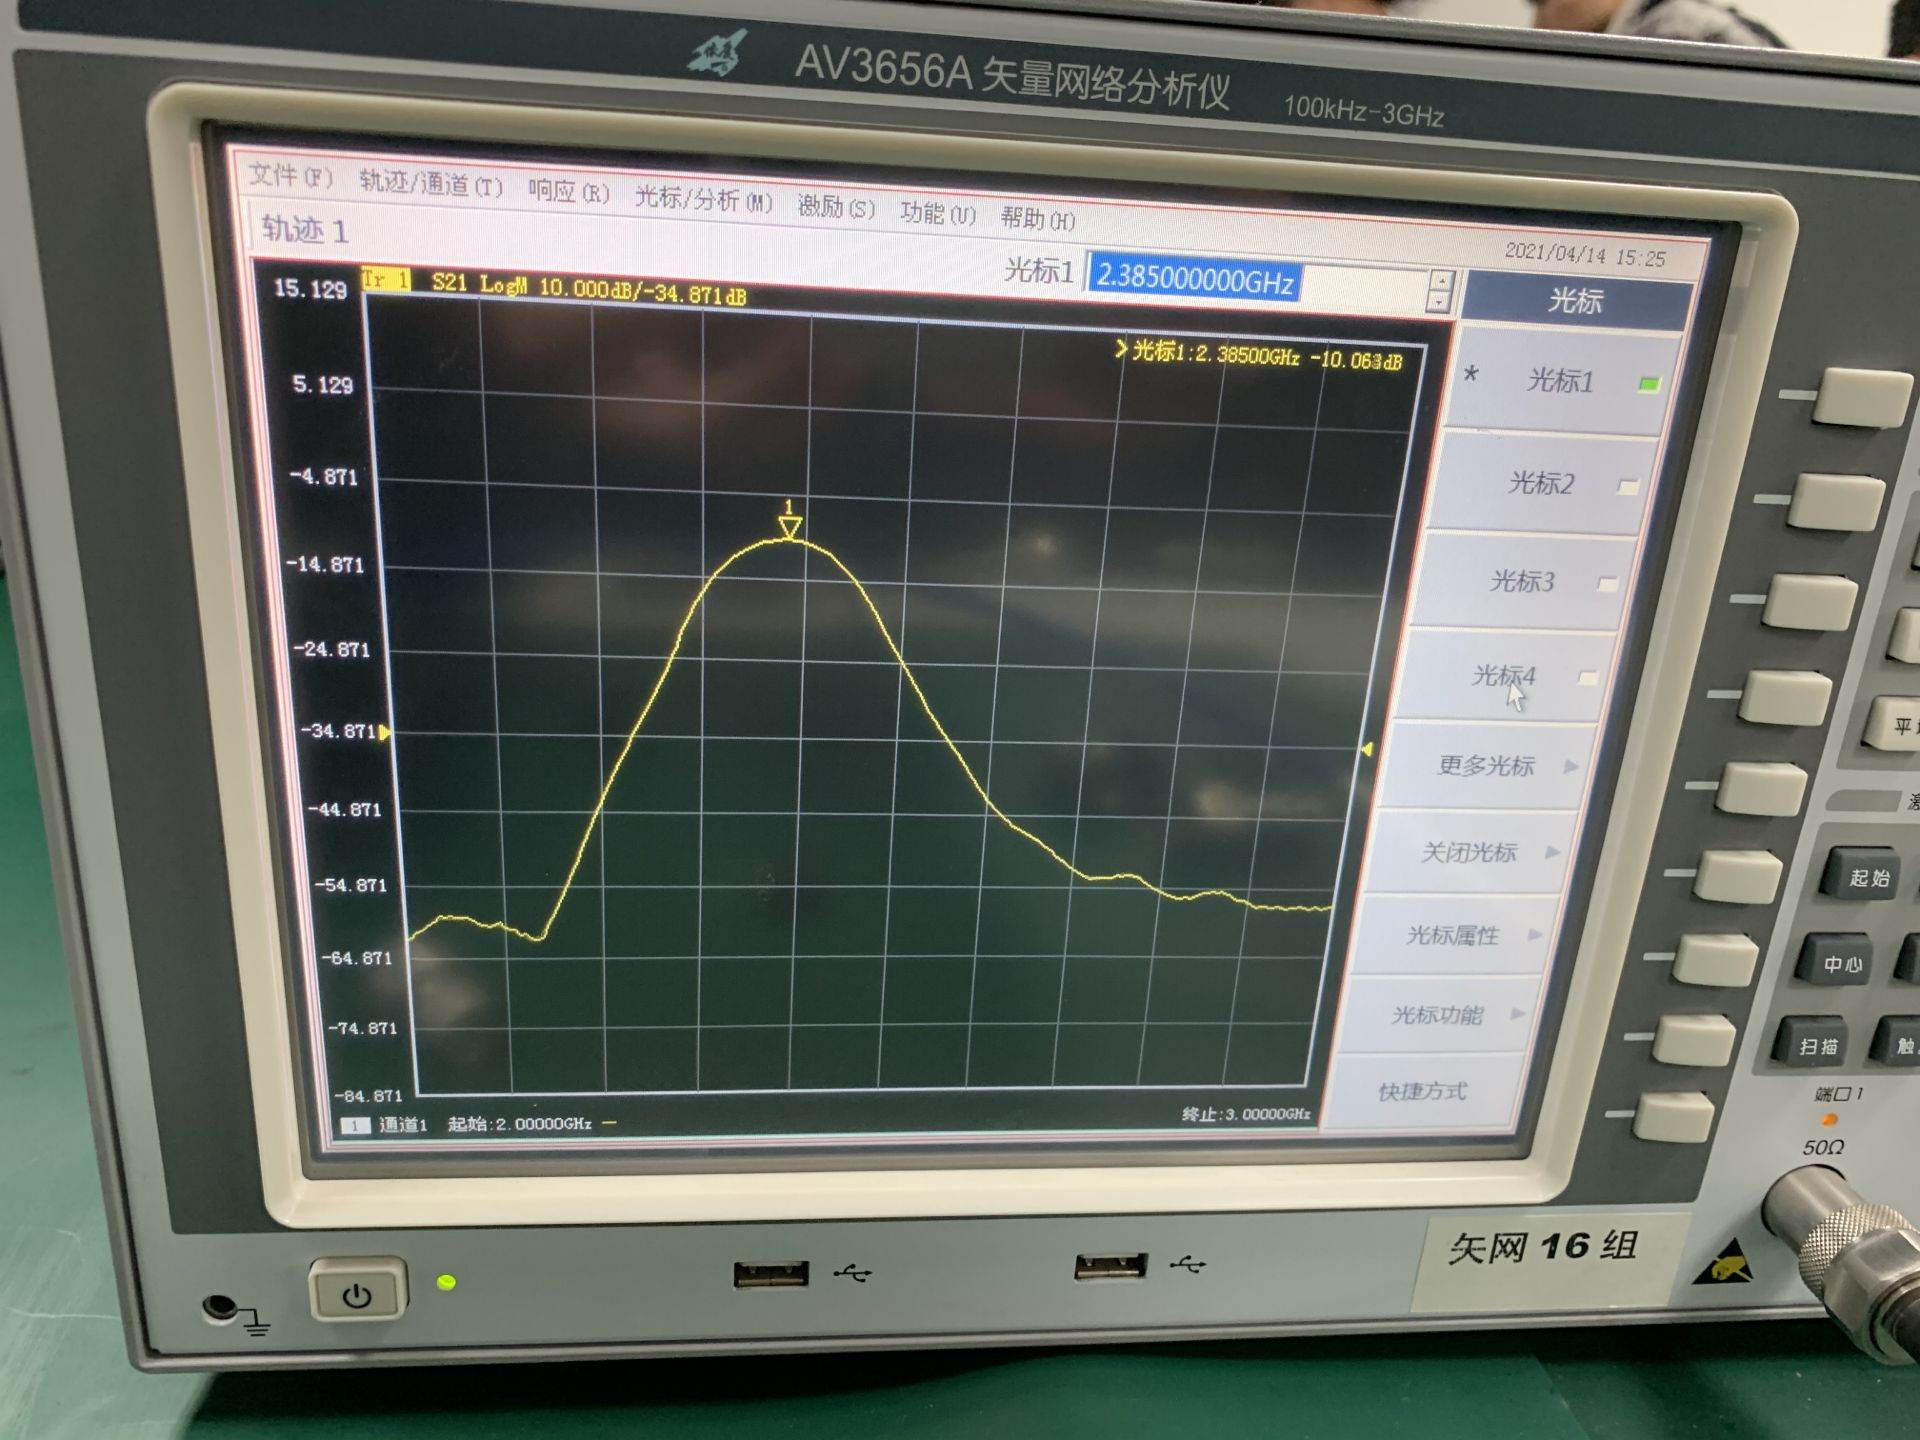
\includegraphics[width=1\textwidth]{pic/滤波特性}
                \caption{$S-w图$}
            \end{minipage}
            \begin{minipage}[t]{0.48\textwidth}
                \centering
                \includegraphics[width=1\textwidth]{pic/相位图}
                \caption{$arg(S)-\omega 图$}
            \end{minipage}
        \end{figure}

        中心频率:2.385GHz
        3dB带宽:114.829MHz
        插入损耗:-10.074dB




    \section{思考题}
        \begin{enumerate}
            \item 什么是S 参数?
            
            S称为散射参数,S12为反向传输系数,也就是隔离。S21为正向传输系数,也就是增益。S11为输入反射系数,也就是输入回波损耗,S22为输出反射系数,也就是输出回波损耗。

            S参数就是建立在入射波、反射波关系基础上的网络参数,适于微波电路分析,以器件端口的反射信号以及从该端口传向另一端口的信号来描述电路网络。同N端口网络的阻抗和导纳矩阵那样,用散射矩阵亦能对N端口网络进行完善的描述。阻抗和导纳矩阵反映了端口的总电压和电流的关系,而散射矩阵是反映端口的入射电压波和反射电压波的关系。散射参量可以直接用网络分析仪测量得到,可以用网络分析技术来计算。只要知道网络的散射参量,就可以将它变换成其它矩阵参量。
            \item 如果不校准,直接接入射频电缆和电路模块测量会对结果有什么影响?
            会使得实验数据测量不准确,呈现出的史密斯圆图不光滑。
            \item 如何测量转接头对测试曲线的影响。
            可以用完全匹配的阻抗进行测试,校准后矢量网络分析仪上距离圆心的距离就是转接头产生的误差。
            \item 利用实验内容2 中已知的设计参数,计算50 欧半波长微带线的长度和宽度。
            
            $$k = \omega \sqrt{\mu \varepsilon _e} = \omega \sqrt{\varepsilon _{re}\varepsilon _0\mu _0} = k_0\sqrt{\varepsilon _{re}}$$
                         $$v_p = \frac{1}{\sqrt{\varepsilon _e\mu _0}} = \frac{1}{\sqrt{\varepsilon _{re}\varepsilon _0\mu _0}} = \frac{c}{\sqrt{\varepsilon _{re}}}$$
                        $$\varepsilon _{re} = \frac{\varepsilon _r + 1}{2} + \frac{\varepsilon _r-1}{2}F(w/h)$$
                        $$Z_e = \frac{\eta _0}{\sqrt{\varepsilon _{re}}}\left\{{\frac{w}{h}+1.393+0.67\mathrm{ln}(\frac{w}{h}+1.44)}\right\}^{-1}$$
                        $$\eta _0 = \sqrt{\mu _0/\varepsilon _0} = 120\pi \Omega $$
得
            $$W = 1.4mm ,\, L = 33mm$$
        \end{enumerate}

    \section{收获与体会}
    通过本次实验,我对理论课上学到的传输线的理论知识理解更加深刻了。也理解到了史密斯圆图在实际实验中的应用。
    \section{实验建议与意见}
    建议提前和将实验的课件发放下来,这样我们好做一些预习,不然就靠上课时的时间很难仓促的理解实验内容。  

      \textsf{latex}  SDfasdfasdfd

\end{document}